\chapter{Basic concepts} \label{chap:concept}
\renewcommand{\tabdir}{chapters/concept/tab}
\renewcommand{\figdir}{chapters/concept/fig}

%%%%%%%%%%%%%%%%%%%%%%%%%%%%%%%%%%%%%%%%%%%%%%%%%%%%%%%%%%%%%%%%%%%%%%%%%%%%%%%%
%%%%%%%%%%%%%%%%%%%%%%%%%%%%%%%%%%%%%%%%%%%%%%%%%%%%%%%%%%%%%%%%%%%%%%%%%%%%%%%%
%%%%%%%%%%%%%%%%%%%%%%%%%%%%%%%%%%%%%%%%%%%%%%%%%%%%%%%%%%%%%%%%%%%%%%%%%%%%%%%%
\section{Important terms} \label{sec:concept-terms}

To understand the concept behind all models created with the \software{echse} simulation environment, one must know the meaning of the terms \emph{class}, \emph{object}, and \emph{object group}. These terms are defined in the following sections (see also  \figref{fig:concept-terms}).

\subsection{Objects} \label{sec:concept-terms-objects}

Objects\index{object!definition} are the basic building blocks of any model created with the \software{echse} simulation environment. An object in the model typically represents a real-world object (such as a tree, a lake, a soil column, etc.). Usually, the object in the model is a simplified, abstract description of the corresponding real-world object, \ie{} it describes only its most important characteristics (for example height, average diameter, and age of a tree). However, an objects does \emph{not necessarily} correspond to an entity existing in the real-world. For example, the function of such a more abstract object may be to simply collect information on some other objects and to supply this information to a third object (like a kind of observer).

Technically speaking, an object always represents an instance of an underlying class (see \secref{sec:concept-terms-classes}). For example, a single tree object is an instance of the tree class. In a typical model, (1) there are multiple instances of the \emph{same} class (such as multiple trees) and (2) multiple objects of \emph{different} classes do co-exist (such as trees and lakes).

The basic features of an object, \ie{} the information and functionality linked to that object, are always determined by the corresponding class (a tree has a diameter and may grow, a lake has a depth and its storage may change). The general features of classes are described in \secref{sec:concept-classFeatures}.

In a typical model, the objects (no matter, of which class) do interact in some way. These interactions typically represent the exchange of matter, energy, or information between the corresponding real-world entities. For example, two lakes could exchange water via a connecting channel or the growth of a tree might depend on a lake's water level.

The collection of all interacting objects is typically called the \emph{model}.

\subsection{Classes} \label{sec:concept-terms-classes}

A class\index{class!definition} represents an abstract prototype for a certain type of object (\emph{type} is an approximate synonym for \emph{class}). A class describes the features of \emph{all} objects that are instances of that particular class. In the language of object-oriented programming, the features of a class are typically called 'class members'. Such member either represent data (\ie{} information) or methods (\ie{} algorithms, describing the functionality of an object of that class). For example, a class 'lake' might have the water level, the storage volume, and the geo-coordinates of its center as data members. These data members (not to be confused with the actual values) are then common to all instances of the class, \ie{} all lake objects.

Generally, a class is distinguished from other classes by
\begin{itemize}
  \item its data members (for example, the number and names of state variables) and/or,
  \item its methods. In the context of the \software{echse}, each class has only a single visible method called 'simulate'. This method typically describes the dynamics of the class' state variables.
\end{itemize}

The members of classes are introduced in detail in \secref{sec:concept-classFeatures}.

\subsection{Object groups} \label{sec:concept-terms-objectgroups}

The term object group\index{object group} is used for all instances (\ie{} objects) of a particular class. If a forest of individual trees is modeled, for example, all trees belong to the same object group. Though, in many instances, the terms \emph{class} and \emph{object group} are (and can be) used synonymously, they are not actually interchangeable:
\begin{description}
  \item [A class] is the prototype of all objects with the same data and functionality.
  \item [An object group] represents the array of all objects (\ie{} instances) of a particular class.
\end{description}

\subsection{Summary} \label{sec:concept-terms-summary}

The relation between the terms \emph{class}, \emph{object}, \emph{object group}, and \emph{model} is illustrated with an example in \figref{fig:concept-terms}. Another view on the relations between these terms is provided in \figref{fig:concept-terms_implementation}. This figure is intended for those who are familiar with basic techniques of object-oriented programming. Shown are 8 objects, which belong to 2 different classes 'A' and 'B'. All these 8 objects inherit from an abstract base class 'abstractObject'. It is therefore possible to keep handles to all these objects (of different classes) in a single array by using base-class pointers (\ie{} by treating them as objects of the base class). In the same way, handles to all object groups can be stored in a single array since they all inherit from an abstract base class 'abstractObjectGroup'. In each object group, an arbitrary number of objects may be declared. In contrast to that, only a single instance of each object group can exist.


\begin{figure}
  \centering
  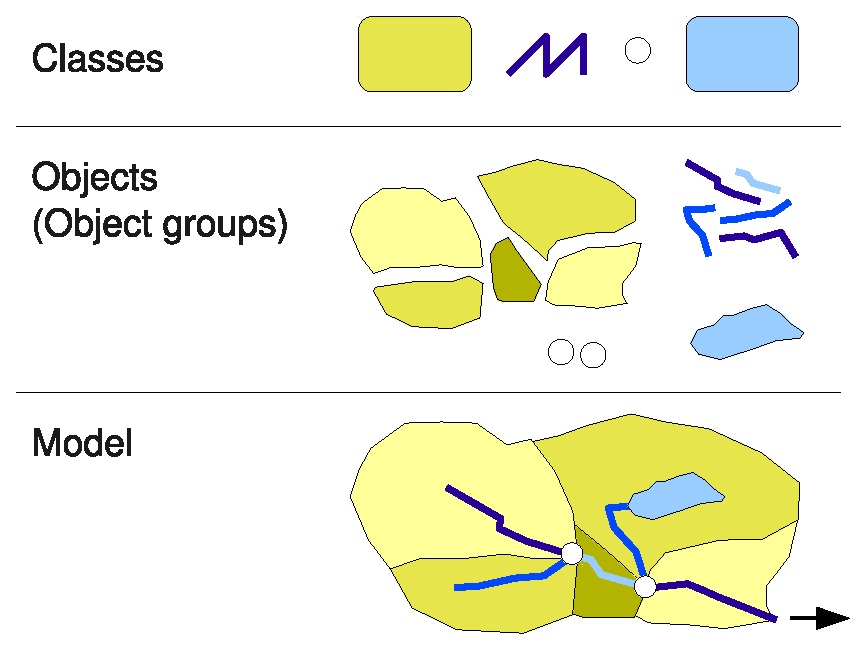
\includegraphics[width=0.9\columnwidth]{\figdir/terms_class-object-objGroup/terms_class-object-objGroup.eps}
  \caption[Relation between the terms \emph{class}, \emph{object}, \emph{object group}, and \emph{model}.]{Relation between the terms \emph{class}, \emph{object}, \emph{object group}, and \emph{model} with the example of a hydrological catchment model, consisting of sub-catchments (green polygons), river reaches (blue lines), lakes (blue polygons), and river nodes (circles). \label{fig:concept-terms}}
\end{figure}

\begin{figure}
  \centering
  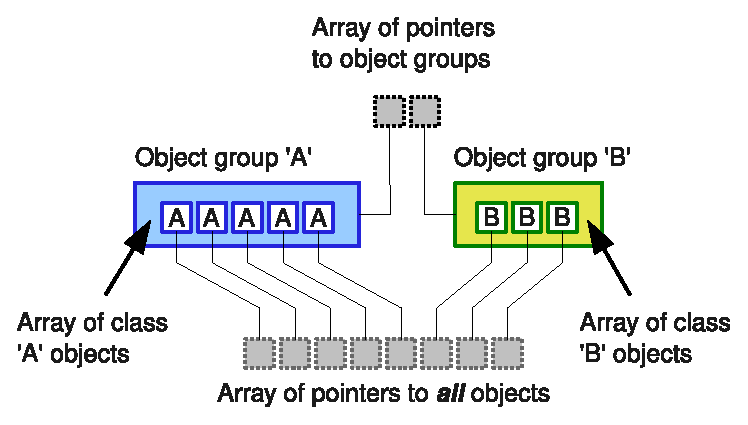
\includegraphics[width=0.9\columnwidth]{\figdir/terms_class-object-objGroup/terms_class-object-objGroup_implementation.eps}
  \caption[\emph{Classes}, \emph{objects}, and \emph{object groups} from a programmers point of view.]{\emph{Classes}, \emph{objects}, and \emph{object groups} from a programmers point of view. \label{fig:concept-terms_implementation}}
\end{figure}

\FloatBarrier

%%%%%%%%%%%%%%%%%%%%%%%%%%%%%%%%%%%%%%%%%%%%%%%%%%%%%%%%%%%%%%%%%%%%%%%%%%%%%%%%
%%%%%%%%%%%%%%%%%%%%%%%%%%%%%%%%%%%%%%%%%%%%%%%%%%%%%%%%%%%%%%%%%%%%%%%%%%%%%%%%
%%%%%%%%%%%%%%%%%%%%%%%%%%%%%%%%%%%%%%%%%%%%%%%%%%%%%%%%%%%%%%%%%%%%%%%%%%%%%%%%
\section{Features (members) of a class} \label{sec:concept-classFeatures}

%%%%%%%%%%%%%%%%%%%%%%%%%%%%%%%%%%%%%%%%%%%%%%%%%%%%%%%%%%%%%%%%%%%%%%%%%%%%%%%%
%%%%%%%%%%%%%%%%%%%%%%%%%%%%%%%%%%%%%%%%%%%%%%%%%%%%%%%%%%%%%%%%%%%%%%%%%%%%%%%%
\subsection{Overview} \label{sec:concept-classFeatures-overview}

An overview of the features (precisely: members\index{class!members}) of a class is given in \figref{fig:concept-classFeatures-overview}. Details on the data members are provided first in \secsref{sec:concept-classFeatures-states} to \ref{sec:concept-classFeatures-outputs}. The 'simulate' method, which is the most important member function of a class, is addressed in \ref{sec:concept-classFeatures-simulateMethod}.

\begin{figure}
  \centering
  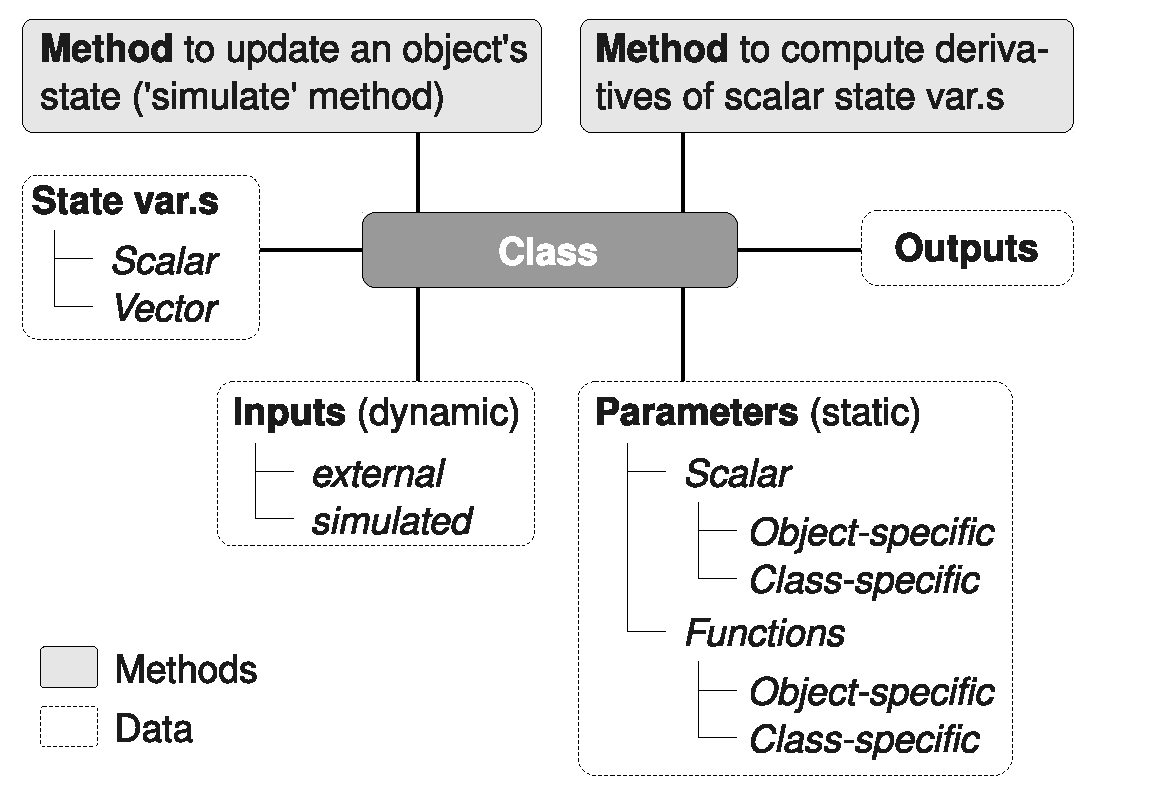
\includegraphics[width=0.9\columnwidth]{\figdir/classFeatures/classFeatures.eps}
  \caption[Overview of the features of a class.]{Overview of the features (members) of a class. The dashed line separates data members (below) from class methods (above line). \label{fig:concept-classFeatures-overview}}
\end{figure}

%%%%%%%%%%%%%%%%%%%%%%%%%%%%%%%%%%%%%%%%%%%%%%%%%%%%%%%%%%%%%%%%%%%%%%%%%%%%%%%%
%%%%%%%%%%%%%%%%%%%%%%%%%%%%%%%%%%%%%%%%%%%%%%%%%%%%%%%%%%%%%%%%%%%%%%%%%%%%%%%%
\subsection{State variables} \label{sec:concept-classFeatures-states}

State variables\index{state variable} describe the state of an object at a certain point in time. State variables are dynamic data, \ie{} their values may change over time. Consequently, at the start of a simulation, their values must be initialized. In \software{echse}-based models, a class may contain both single-valued (scalar) and vector-valued state variables.

\subsubsection*{Scalar state variables} \label{sec:concept-classFeatures-statesScal}

\emph{Scalar state variables}\index{state variable!scalar} are state variables that take a single value only. Looking at a reservoir, for example, the storage volume is a scalar state variables, since it can be expressed as a single number. In contrast to that, the reservoirs' water depth (as it is spatially variable) is not a scalar variable by nature. The average depth, however, may be treated as a scalar state variable.

\subsubsection*{Vector state variables} \label{sec:concept-classFeatures-statesVect}

In contrast to a scalar state variables, \emph{vector state variables}\index{state variable!vector-valued} are vector-valued, \ie{} their value(s) cannot be adequately expressed by a single number. For example, a vector state variable may be required to adequately describe the temperature in a deep reservoir. Due to stratification, there are often significant vertical temperature gradients which often cannot be (convieniently) described by a single value (\ie{} a scalar state variable). Another example of a vector state variable is the water level of a river reach, measured at multiple stations along that reach.

%%%%%%%%%%%%%%%%%%%%%%%%%%%%%%%%%%%%%%%%%%%%%%%%%%%%%%%%%%%%%%%%%%%%%%%%%%%%%%%%
%%%%%%%%%%%%%%%%%%%%%%%%%%%%%%%%%%%%%%%%%%%%%%%%%%%%%%%%%%%%%%%%%%%%%%%%%%%%%%%%
\subsection{Input variables} \label{sec:concept-classFeatures-inputs}

Input variables (also called forcings)\index{input variable} represent time-variable data, representing the dynamic environment of an object. Typically, changes in the values of an object's state variables are triggered by changes in the input variables. In \software{echse} models, \emph{external} and \emph{simulated} (synonym: internal) inputs are distinguished.

%%%%%%%%%%%%%%%%%%%%%%%%%%%%%%%%%%%%%%%%%%%%%%%%%%%%%%%%%%%%%%%%%%%%%%%%%%%%%%%%
\subsubsection*{External inputs} \label{sec:concept-classFeatures-inputsExt}

External input variables\index{external input}\index{input variable!external|see{external input}}\index{forcing|see{external input}}\index{boundary condition|see{external input}} are variables, whose dynamics is \emph{not} simulated by the model. Instead, the dynamics is prescribed, \ie{} the values must be known in advance for the entire modeling period. The model reads those data from time series files (see \secref{sec:input-external}). When simulating the temperature of a reservoir, for example, solar radiation and air temperature are typically external input variables (since the atmosphere itself is not part of the model). Values of the external input variables usually represent observations (when simulating the past). In the context of forecasting, the values often originate from forecasts which have been produced by an external model. For example, a hydrological model for medium-term stream flow forecasting uses the forecasts produced by a numerical weather prediction model as input.

%%%%%%%%%%%%%%%%%%%%%%%%%%%%%%%%%%%%%%%%%%%%%%%%%%%%%%%%%%%%%%%%%%%%%%%%%%%%%%%%
\subsubsection*{Simulated inputs} \label{sec:concept-classFeatures-inputsSim}

The values of simulated input variables\index{simulated input}\index{input variable!simulated|see{simulated input}} are computed \emph{within} the model itself. From the perspective of an object, a simulated input variable is a variable, whose values are supplied by another object, \ie{} the existence of such variables is bound to interactions between objects. More precisely, a simulated input variable of an object 'A' is always linked to an output variable (see \secref{sec:concept-classFeatures-outputs}) of another object 'B'. This is due to the fact that only the output variables of an object are visible to (and accessible by) other objects. A typical example for the use of simulated inputs is the 'reservoir' class in a hydrological model. From the perspective of a reservoir, the inflow is a simulated input variable, if the values are supplied by an upstream object. The corresponding output variable of the upstream object is usually an outflow rate (of a reach) or a runoff rate (from the reservoir's catchment).

%%%%%%%%%%%%%%%%%%%%%%%%%%%%%%%%%%%%%%%%%%%%%%%%%%%%%%%%%%%%%%%%%%%%%%%%%%%%%%%%
%%%%%%%%%%%%%%%%%%%%%%%%%%%%%%%%%%%%%%%%%%%%%%%%%%%%%%%%%%%%%%%%%%%%%%%%%%%%%%%%
\subsection{Parameters} \label{sec:concept-classFeatures-params}

Those properties of an object which are static (\ie{} which do not change over time), are called \emph{parameters}\index{parameter}. As outlined in \figref{fig:concept-classFeatures-overview}, different kinds of parameters are supported by the \software{echse}. These are described in detail in the subsequent sections.

%%%%%%%%%%%%%%%%%%%%%%%%%%%%%%%%%%%%%%%%%%%%%%%%%%%%%%%%%%%%%%%%%%%%%%%%%%%%%%%%
\subsubsection*{Scalar parameters} \label{sec:concept-classFeatures-paramsNum}

\emph{Scalar parameters}\index{parameter!scalar} are, like scalar state variables, characterized by the fact that they are single-valued. Thus, the value of a scalar parameter is always just a single number. In the \software{echse}, two types of scalar parameters are distinguished:
\begin{description}
  \item [Object-specific scalar parameters]: The value of these parameters are specific for a particular object (of a particular class). For example, a 'catchment' class could have an object-specific scalar parameter 'area'. Then, values of the area may be assigned to each catchment object individually.
  \item [Group-specific scalar parameters]: The value of such a parameter cannot be set for individual objects. Instead, a common value is assigned to \emph{all} objects of a particular class. For example, in a 'catchment' class, the long-wave emissivity of the snow cover could be declared as a group-specific scalar parameter, if a common value for all modeled catchments is appropriate.
\end{description}

Note: Hard-coded scalar parameters, \ie{} the definition of constants in the 'simulate' method of a class, provide(s) an alternative to group-specific scalar parameters. The use of hard-coded parameters is preferable \emph{only} if it is known that the values are strictly constant. This is typically the case for physical constants with a well known value (such as the specific heat capacity of water). The drawback of using hard-coded parameters is that any modification of the values requires the source code to be re-compiled. Note that, strictly speaking, such hard-coded parameters are not \emph{data members} of the class and, therefore, they do not show up in \figref{fig:concept-classFeatures-overview}.

%%%%%%%%%%%%%%%%%%%%%%%%%%%%%%%%%%%%%%%%%%%%%%%%%%%%%%%%%%%%%%%%%%%%%%%%%%%%%%%%
\subsubsection*{Parameter functions} \label{sec:concept-classFeatures-paramsFun}

In many situations, some static object properites need to be represented by functions\index{parameter!function} instead of scalar parameters. An example is the relationships between water depth and storage volume in a river reach or lake. The \software{echse} basically supports two concepts of functions:
\begin{enumerate}
  \item Tabulated functions (synonym: lookup tables).
  \item Analytical expressions.
\end{enumerate}

\paragraph{Tabulated functions:} Lookup tables provide a means to describe also those functional relations between two entities which cannot be reasonably captured by an analytical expression. Although, in many cases, a piecewise polynomial representation might be possible, lookup tables offer a more flexible and convenient alternative. The \software{echse} supports tabulated functions as long they have a single argument only. There is support for both functions with regular (\ie{} equally spaced) arguments and functions with non-regular arguments. Like in the case of scalar parameters, two types of such lookup-based parameter functions may be distinguished:

\begin{description}
  \item [Object-specific parameter functions]: This type of function is object-specific, \ie{} an individual lookup table is assigned to each object (of a particular class). For example, the rating curve might be declared as an object-specific parameter function in a 'gage' class, since each gage has its own characteristic rating curve.
  \item [Group-specific parameter functions]: Such a function is not associated with an individual object. Instead, it represents a common function which is accessible to all objects (of a particular class).
\end{description}

\paragraph{Analytical expressions:} If a function can be captured by a single (or few) analytical expression(s), then it is typically hard-coded, \ie{} the function is defined in the 'simulate' method of a class. It is then, strictly speaking, not a \emph{data member} of the class and, therefore, hard-coded functions do not show up in \figref{fig:concept-classFeatures-overview}. Hard-coded analytical functions include, for example, polynomials, and linear, exponential, or power functions. The advantage of using them is that the function's return value may usually be computed more quickly as compared to table-lookup.

A typical case of an analytical function that one would hard-code is the Magnus-Formula, which is is an empirical expression relating the air's maximum humidity to air temperature. It is an example of a function which is \emph{not} object-specific since it is practically applicable everywhere on earth.

However, it is quite straightforward to make hard-coded functions object-specific. This is simply achieved by passing the coefficients of analytical expressions via the functions interface and to define those coefficients as object-specific \emph{scalar parameters}. For example, a rating curve may sometimes be expressed by a power expression like $Q=a \cdot H^b$, with $a$ and $b$ being empirical coefficients and $Q$ and $H$ representing discharge and stage, respectively. In such a case, one may declare $a$ and $b$ as object-specific \emph{scalar} parameters in a 'gage' class to let each gages have its individual rating curve.

Note that hard-coded analytical functions provide the only way of implementing functions that take multiple variable arguments (multi-dimensional functions). This is due to the fact that there is currently no support for multi-dimensional table lookup. In some situations, however, it may be possible to split a multi-dimensional function into several single-argument functions which may then be represented by lookup tables.

%%%%%%%%%%%%%%%%%%%%%%%%%%%%%%%%%%%%%%%%%%%%%%%%%%%%%%%%%%%%%%%%%%%%%%%%%%%%%%%%
%%%%%%%%%%%%%%%%%%%%%%%%%%%%%%%%%%%%%%%%%%%%%%%%%%%%%%%%%%%%%%%%%%%%%%%%%%%%%%%%
\subsection{Output variables} \label{sec:concept-classFeatures-outputs}

To make information about an object visible to (and usable for) its environment, \emph{output variables}\index{output variable} must be declared in the respective class. In particular, output variables have to be declared in a class for all data, which
\begin{itemize}
  \item should to be passed from an object of that class to another simulated object.
  \item are of interest to the modeler and should (potentially) be available in the output files.
\end{itemize}

In a hydrological catchment model, for example, a 'catchment' class might have an output variable 'runoff'. Then, the values of that variable may serve as an input to an object of class 'reach', for example, provided that a corresponding \emph{simulated input} variable (see \secref{sec:concept-classFeatures-inputsSim}) exists in the 'reach' class. Furthermore, the existance of the output variable 'runoff' allows for writing the computed runoff for user-selected catchments to the respective output files.

In each class, at least a single output variable should be defined because objects of that class are otherwise useless. Typically, output variables are used to retrieve information on
\begin{itemize}
  \item state variables.
  \item flux rates, such as time-step averages of energy or mass fluxes.
\end{itemize}
However, there are practically no limitations, \ie{} any scalar value which is computed (or which is accessible) in the 'simulate' method of a class (see \secref{sec:concept-classFeatures-simulateMethod}) can be assigned to an output variable.

%%%%%%%%%%%%%%%%%%%%%%%%%%%%%%%%%%%%%%%%%%%%%%%%%%%%%%%%%%%%%%%%%%%%%%%%%%%%%%%%
%%%%%%%%%%%%%%%%%%%%%%%%%%%%%%%%%%%%%%%%%%%%%%%%%%%%%%%%%%%%%%%%%%%%%%%%%%%%%%%%
\subsection{The 'simulate' method} \label{sec:concept-classFeatures-simulateMethod}

\subsubsection*{Purpose and interface}
The 'simulate' method\index{simulate method} of a class represents the class' most important member function which needs to be defined by the model developer.

The purpose of the 'simulate' method is to simulate the evolution of an object over a period of length $\Delta t$. This is usually equivalent to solving a so-called \emph{initial value problem} which means that

\begin{enumerate}
  \item the values of the object's $n$ state variables at an initial time $t_0$ are known.
  \item the values at time $t_0 + \Delta t$ are to be computed by integrating $n$ ordinary differential equations (one ODE per state variable).
\end{enumerate}

Thus, the 'simulate' method usually implements a solution of the initial value problem. The ordinary differential equations (ODEs) to be solved are specific for each class and they typically describe either a mass or energy balance (see example in \secref{sec:concept-classDef}). Whether the integration can be performed using simple approaches (such as a first order Euler method) or whether sophisticated ODE solvers \citep[see \eg{}][]{Press2002} are required, depends on the specific problem. In addition to the updating of state variables, the 'simulation' method is responsible for calculating all auxiliary numeric data, which are of interest to the model user, \ie{} model outputs (see \secref{sec:concept-classFeatures-outputs}).

In C++ notation, the interface of the 'simulate' method looks like

\medskip
{\small \verb!.simulate(const unsigned int delta_t)!}
\medskip

where \verb!delta_t! is the function's (only) argument. It is of type unsigned integer and represents the simulation time step in seconds. Note that no other information are passed via the function's argument list.

\subsubsection*{Class-specific behavior}
The leading dot in the function's name (see interface above) indicates that this function is a class member. Formally speaking, it is a \emph{virtual} member of the \emph{abstract} class 'abstractObject' describing a generic object (\figref{fig:concept-simulateMethod}). The child classes describing a specific type of (usually real-world) objects are derived from that abstract parent class. Through the mechanisms of inheritance, each child class automatically has a 'simulate' method with the interface shown above. Although the function's name is the same, the interior of the method is \emph{class-specific}, since the implementation is only present in the child classes but not in the base class (\figref{fig:concept-simulateMethod}). This makes it possible to use identical calls like

\medskip
{\small \verb!reservoir_xy.simulate(3600)!}

{\small \verb!catchment_288.simulate(3600)!}
\medskip

to trigger the simulation of two objects, which are instances of \emph{different} classes (a 'reservoir' and a 'catchment', in this example). The appropriate code for each object is selected automatically at run-time, based on the type information.

\begin{figure*}[htb]
\lstinputlisting[style=c++]{\figdir/simulate-methods/simulate-methods.txt}
  \caption[Specification of the 'simulate' methods in the abstract base class (parent class) and the application-specific child classes.]{Specification of the 'simulate' methods in the abstract base class (parent class) and the application-specific child classes. Only relevant parts of the C++ code of the classes are shown. \label{fig:concept-simulateMethod}}
\end{figure*}

\subsubsection*{Access to an object's data}

As mentioned earlier, the time step \verb!delta_t! is the only information passed to the 'simulate' method via the argument list. All object-related data, such as the values of parameters, inputs, and state variables, are available through class methods. These methods, which may also be called \emph{data access methods}, are summarized in \tabsref{tab:concept-dataAccessFunctions_read} and \ref{tab:concept-dataAccessFunctions_write}.

The read-only methods (\tabref{tab:concept-dataAccessFunctions_read}) are intended for retrieving information. They can appear at the right-hand side of assignments and the methods with a scalar result type may be used in mathematical expressions or comparisons just like normal variables of type \verb!double!. The method for retrieving the values of a vector state variable does not return a scalar result but a constant reference to a numeric vector (\verb!const vector <double> &!). Note that it depends on the \emph{usage} of the return value whether a copy of the retrieved data is generated or not. This is important in terms of computational efficiency if the vectors are large size. To avoid the creation of a copy, you have to use the returned value to initialize a const reference. In C++, this would look like

\medskip
\begin{footnotesize}
  \verb!const vector <double> & = stateVect(name);!
\end{footnotesize}
\medskip

where \verb!name! is the name of the respective vector state variable. If you assign the return value to a 'normal' variable, \ie{} a non-constant numeric vector which is not a reference, using

\medskip
\begin{footnotesize}
  \verb!vector <double> = stateVect(name);!
\end{footnotesize}
\medskip

a copy of the data will be created. Note that this distinction is also relevant when passing the vector to a function via the function's argument list. Since you often want to pass a constant reference instead of a copy of the values, the dummy argument should be declared accordingly.

The purpose of the write-only methods (\tabref{tab:concept-dataAccessFunctions_write}) is to assign new values to an object's state or output variables (see example in \secref{sec:concept-classDef}). The write-only methods all return non-const references to scalars or vectors. These methods typically appear at the left-hand side of assignment statements. They may also be used as actual parameters in function calls, if the corresponding template parameter is a non-const reference of the appropriate type (\ie{} the parameter represents an output of the function).

\begin{table*}[htb]
  \caption[Data access methods, part I: Read-only methods.]{Data access methods, part I: Read-only methods. The dummy argument \texttt{name}, has to be substituted by the name of the particular variable, parameter, or function to be accessed. The names are defined by the model developer. Note that names must not be quoted since they do not represent strings but (automatically defined) index constant. For the dummy argument \texttt{arg}, a numeric expression representing the function's argument has to be supplied. \label{tab:concept-dataAccessFunctions_read}}
  \begin{tabular}{p{0.18\textwidth}ll} \hline\hline
    Type of feature       & Call                   & Result type \\ \hline
    Scalar state variable & \verb!stateScal(name)! & \verb!double! \\
    Vector of scalar state variables & \verb!stateScal_all()! & \verb!const vector <double> &! \\
    Vector state variable & \verb!stateVect(name)! & \verb!const vector <double> &! \\
    External input    & \verb!inputExt(name)! & \verb!double! \\
    Simulated input   & \verb!inputSim(name)! & \verb!double! \\
    Parameter function (object-specific) & \verb!paramFun(name, arg)! & \verb!double! \\
    Scalar parameter (object-specific) & \verb!paramNum(name)! & \verb!double! \\
    Parameter function (group-specific) & \verb!sharedParamFun(name, arg)! & \verb!double! \\
    Scalar parameter (group-specific) & \verb!sharedParamNum(name)! & \verb!double! \\
    \hline\hline
  \end{tabular}
\end{table*}

\begin{table*}[htb]
  \caption[Data access methods, part II: Write-only methods.]{Data access methods, part II: Write-only methods. See \tabref{tab:concept-dataAccessFunctions_read} for details on the methods' \texttt{name} argument. \label{tab:concept-dataAccessFunctions_write}}
  \begin{tabular}{p{0.3\textwidth}ll} \hline\hline
    Type of feature & Call & Assigned type \\ \hline
    Scalar state variable & \verb!set_stateScal(name)! & \verb!double &! \\
    Vector of scalar state variables & \verb!set_stateScal_all()! & \verb!vector <double> &! \\
    Vector state variable & \verb!set_stateVect(name)! & \verb!vector <double> &! \\
    Output variable & \verb!set_output(name)! & \verb!double &! \\
    \hline\hline
  \end{tabular}
\end{table*}

\subsubsection*{Mandatory actions}
According to the purpose of the 'simulate' method (see above), there is a minimum set of statements that should be present in this method for every class (see example in \secref{sec:concept-classDef}). In particular, the method should contain
\begin{enumerate}
  \item statements to update the values of all state variables using the method(s) from row 1 \& 2 of \tabref{tab:concept-dataAccessFunctions_write}. As discussed earlier, this usually means that ordinary differential equations are solved (see also \secref{sec:concept-classFeatures-derivsScal}).
  \item statements to set the values of all output variables (see last row of \tabref{tab:concept-dataAccessFunctions_write}).
\end{enumerate}

%%%%%%%%%%%%%%%%%%%%%%%%%%%%%%%%%%%%%%%%%%%%%%%%%%%%%%%%%%%%%%%%%%%%%%%%%%%%%%%%
%%%%%%%%%%%%%%%%%%%%%%%%%%%%%%%%%%%%%%%%%%%%%%%%%%%%%%%%%%%%%%%%%%%%%%%%%%%%%%%%
\subsection{The 'derivsScal' method} \label{sec:concept-classFeatures-derivsScal}
As described in \secref{sec:concept-classFeatures-simulateMethod}, the purpose of the 'simulate' method is usually to integrate a single (or a set of) ordinary differential equation(s) over time. In some situations, the use of a simple first-order approximation (Euler's method) may be sufficient. Such methods, however, are neither accurate nor stable. If more accurate and stable solutions are needed, an ODE solver must be used which yields higher-order estimates and automatically adjusts the size of time (sub)steps.

The \software{echse} comes with a built-in ODE solver based on the 5-th order Runge-Kutta method described in \citet{Press2002}. This is a quite robust algorithm. However, its applicability is restricted to \emph{non-stiff} systems of simultaneous ODE. This may be relevant if the number of state variables of an object is > 1.

As with all ODE solvers, one must pass a method to the solver which computes the derivatives of the state variables (with respect to time, here). The name of the corresponding class method is 'derivsScal'. Like 'simulate', it is a virtual method. As the method's name indicates, it computes the derivatives of the scalar state variables only (see \secref{sec:concept-classFeatures-statesScal}). ODE solver support for vector state variables is currently not implemented.

The interface of the 'derivsScal' method is shown in \figref{fig:concept-classDef-methodsFrame}. The meaning of the dummy arguments is as follows:

\begin{tabular}{lp{0.8\columnwidth}}
  \verb!t! & This scalar \emph{input} argument represents the time. It is only relevant when simulating non-autonomous systems, \ie{} if the value(s) of the derivative(s) are time-depend. Note that this is only the case, if the forcings are variable within a time step. In many models, the forcings are treated as constant within a time step and the value of \verb!t! is not used in computing the derivatives. \\
  \verb!u! & \emph{Input} vector holding the values of the state variables whose derivatives are to be computed. \\
  \verb!dtdt! & \emph{Output} vector, containing the derivatives corresponding to the state variables in \verb!u!. \\
  \verb!delta_t! & \emph{Input} value, representing the length of the simulation time step. The intention of this argument is to allow for unit conversions. For example, external forcings (precipitation, radiation) may be given as sum values for a time step (mm/time step or J/\sqm{}/time step, for example). When computing the derivatives, such values need to be converted into rates (m/s or W/\sqm{}, for example) using the value of \verb!delta_t!. \\
\end{tabular}

In order to actually use this method, the code for computing the derivatives needs to provided in a separate file (see \verb!#include! directive in the 'derivsScal' method in \figref{fig:concept-classDef-methodsFrame}). This file must contain code which assigns a value to all elements of vector \verb!dudt!. At the right hand side of these assignments, one can use the access functions listed in \tabref{tab:concept-dataAccessFunctions_read} with one \emph{important exception}: One \emph{cannot} call the function \verb!stateScal! to access the value(s) of scalar state variable(s)! Instead, one must use the respective element of the input vector \verb!u! (appropriate constants for accessing a particular element are provided in the generated class header). This is because of the fact that the ODE solver internally computes derivatives for various estimates of the state variables' values. These estimates are passed in vector \verb!u!. Note that the body of the 'derivsScal' method can remain empty if there is no need for it (because the ODE(s) can be solved analytically, for example).

See \secref{sec:concept-classDef-simulate} for an example showing an implementation of the 'derivsScal' method and the use of the built-in ODE solver in the 'simulate' method.

%%%%%%%%%%%%%%%%%%%%%%%%%%%%%%%%%%%%%%%%%%%%%%%%%%%%%%%%%%%%%%%%%%%%%%%%%%%%%%%%
%%%%%%%%%%%%%%%%%%%%%%%%%%%%%%%%%%%%%%%%%%%%%%%%%%%%%%%%%%%%%%%%%%%%%%%%%%%%%%%%
%%%%%%%%%%%%%%%%%%%%%%%%%%%%%%%%%%%%%%%%%%%%%%%%%%%%%%%%%%%%%%%%%%%%%%%%%%%%%%%%

\FloatBarrier

\section{Automatic code generation} \label{sec:concept-autocode}

\subsection{Role of generated code in the \software{echse} framework} \label{sec:concept-autocode-role}
As stated in \chapref{chap:intro}, the \software{echse} is a generic modeling framework. As such, it consists of a generic, re-usable model core complemented by problem-specific extensions. The generic model core provides basic infrastructure for \emph{any} dynamic simulation model. The problem-specific extensions are required to build simulation models for a particular (type of) system.

In the case of the \software{echse} modeling framework, problem-specific extensions are equivalent to user-defined classes with the features described in \secref{sec:concept-classFeatures}. The relation between the generic model core and the problem-specific extensions is illustrated in \figref{fig:concept-autocode-role}.

\begin{figure}
  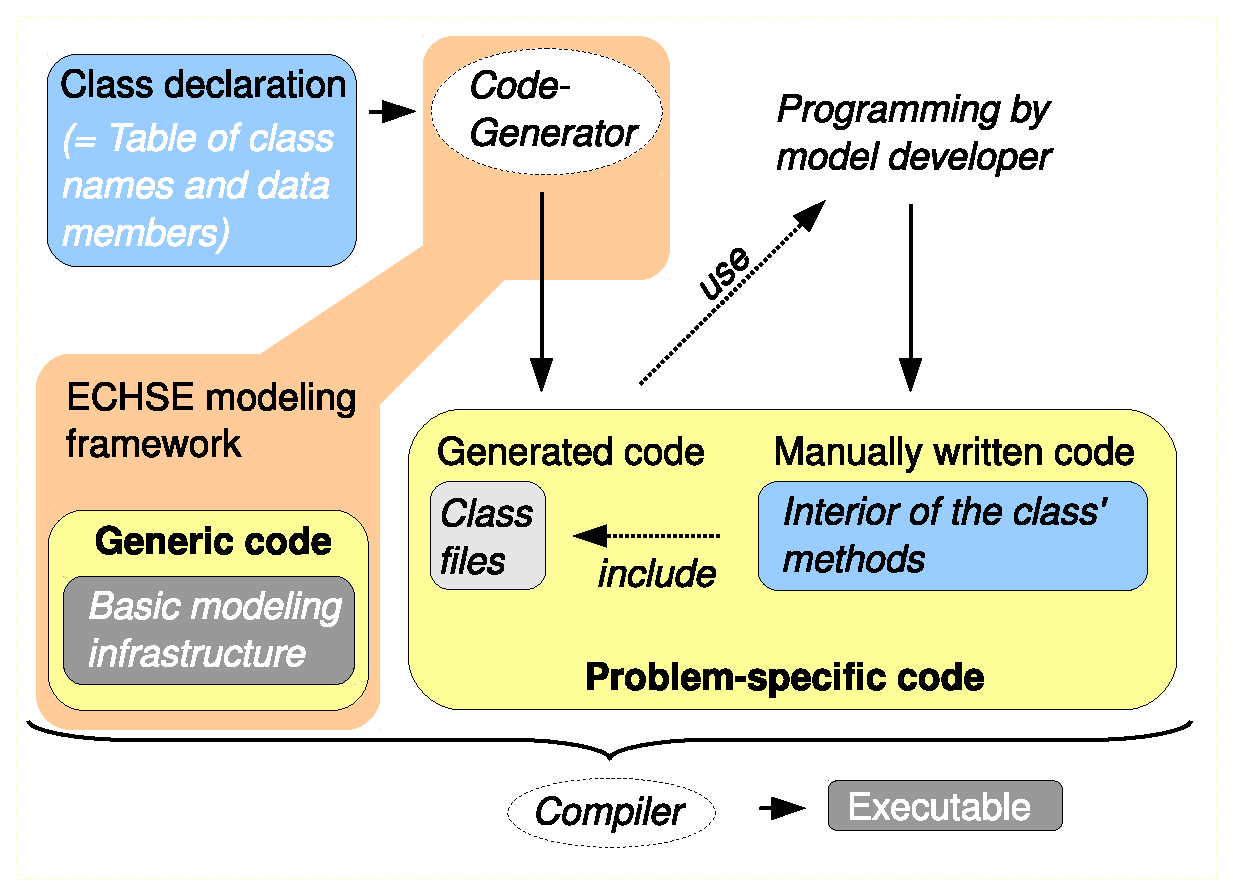
\includegraphics[width=0.9\columnwidth]{\figdir/echseIdea/echseIdea.eps}
  \caption{Major components of the \software{echse} modeling framework. \label{fig:concept-autocode-role}}
\end{figure}

To sucessfully build a simulation model with the \software{echse} framework, the problem-specific part of the source code (class definitions) must be perfectly compatible with the generic model core on the one hand. On the other hand, good practice of software development requires that the generic core and the problem specific extensions are well separated. In fact, a developer who implements the problem-specific classes should not need to understand or even know any details of the generic core.

In the \software{echse} modeling framework, this dilemma is solved by means of automatic source code generation (\figref{fig:concept-autocode-role}). In this concept, the model developer first \emph{declares} a class by specifying the names and types of all data members (see \figref{fig:concept-classFeatures-overview} for possible member types). In a second step, a program automatically generates the class' basic source code from the provided declaration. This generated code is guaranteed to be compatible with the generic core. It provides entry points for additional source code which has to be manually written in a third step. This manually written code comprises the bodies of the 'simulate' and the 'derivsScal' methods (see \secsref{sec:concept-classFeatures-simulateMethod} and \ref{sec:concept-classFeatures-derivsScal}).

The three steps of
\begin{enumerate}
  \item Declaration of data members
  \item Code generation
  \item Implementation of methods
\end{enumerate}
are illustrated in \secref{sec:concept-classDef} with the example of a linear reservoir class.

The advantages of the strategy of automatic code generation can be summarized as follows:
\begin{itemize}
  \item The model developer does not need to manually write all the abstract code related to the classes and the corresponding object groups (recall \secref{sec:concept-terms-summary}). This reduces development times for new models.
  \item The model developer does not need to care for the compatibility of the application-specific code with the code forming the generic core of any \software{echse} model. This makes model development really a simple and save task.
\end{itemize}

\subsection{The code generator} \label{sec:concept-autocode-codegen-basic}

\index{code generator}

\subsubsection*{Installation}
The code generator is currently implemented in the R programming language. It is contained in the R-package \software{codegen} which provides a single method whose name is \texttt{generate}. The package is provided as a tarball with name \verb!codegen_x.y.tar.gz! where x.y is a version number. See \citet{Echse-Install-Doc} for details on how to install the R software and add-on packages. The \software{codegen} package depends on no other packages.

\subsubsection*{Standard documentation}
After the \software{codegen} package has been loaded, for example using the R command

\begin{lstlisting}[style=R]
library("codegen")
\end{lstlisting}

the documentation of the \texttt{generate} method can be displayed by typing the question mark followed by the method's name.

\begin{lstlisting}[style=R]
?generate
\end{lstlisting}

\subsubsection*{Examples}
To run an illustrative example, one can use the following R command.

\begin{lstlisting}[style=R]
example("generate")
\end{lstlisting}

It generates sample input files for the \texttt{generate} method and then runs the method on these files. Another practical example, can be found in \secref{sec:concept-classDef}.

\subsection{Inputs of the code generator} \label{sec:concept-autocode-codegen-input}

The code generator assumes that each class is declared in a \emph{separate} file. Such a class declaration file must be a plain, TAB-separated text file with two columns 'type' and 'name' (see \figref{fig:concept-classDef-declaration-example} for an example). Each record in this table declares a single data member of the class. The meaning of the two columns is as follows:

\begin{columndef}
  \item [type] (\textit{string}) The type of the feature to be declared. Valid entries are listed in \tabref{tab:concept-featuretypes}.
  \item [name] (\textit{string}) The name of the variable, parameter, or function to be declared. The name must be a valid C++ identifier.
\end{columndef}

In addition to these two mandatory columns, the table may have additional columns which are ignored during processing by the code generator. For the purpose of documentation, it is recommended to append at least one column with a short description of each feature and probably the physical units. Moreover, the file may contain comment lines starting with the \verb!#! character (see example in \figref{fig:concept-classDef-declaration-example}). It may be  convenient to prepare the table in a spreadsheet software first and to save the contents to a text file later (by copy \& paste, for example).

\begin{table}[htb]
  \caption[Description of the keywords expected in the 'type' column of a class declaration table.]{Description of the keywords expected in the 'type' column of a class declaration table (see example in \figref{fig:concept-classDef-declaration-example}). \label{tab:concept-featuretypes}}
  \begin{tabularx}{\columnwidth}{lX} \hline\hline
    Keyword & Type of feature \\ \hline
    \texttt{stateScal} & Scalar state variable \\
    \texttt{stateVect} & Vector state variable \\
    \texttt{inputExt} & External input variable \\
    \texttt{inputSim} & Simulated input variable \\
    \texttt{paramNum} & Object-specific scalar parameter \\
    \texttt{sharedParamNum} & Group-specific scalar parameter \\
    \texttt{paramFun} & Object-specific parameter function \\
    \texttt{sharedParamFun} & Group-specific parameter function \\
    \texttt{output} & Output variable \\
    \hline\hline
  \end{tabularx}
\end{table}

\subsection{Outputs of the code generator} \label{sec:concept-autocode-codegen-output}

The code generator produces several C++ header files (file extension '.h'). The individual files are only briefly described here. The files' contents is not shown.
\begin{description}
  \item [Instantiation function definition file] This file contains a function which, when called, creates a single instance of each object group based on class template. The function returns a handle to the object groups (in the form of a pointer vector).
  \item [Header bundle file] This file contains C++ include statements, referencing all header files created by the code generator, except for the file itself. This provides a means to include a variable (application-specific) number of header files into the generic source files without the need for any modification there.
  \item [Class header file(s)] For each class declared by the model developer, a header file is generated. It describes the abstract prototype of an object of the respective class. Note that the implementation of the class' methods 'simulate' or 'derivsScal' are  \emph{not} contained here. Instead, references to include files are generated and these include files must be manually filled with code by the model developer.
  \item [Index constants file(s)] For each class declared by the model developer, a file with index constants is created. These index constants must be used when querying or manipulating an object's data via the methods described in \tabsref{tab:concept-dataAccessFunctions_read} and \ref{tab:concept-dataAccessFunctions_write}. The automatically defined constants allow for referencing a particular variable, parameter, or function \emph{by name} (see the 'name' argument in \tabref{tab:concept-dataAccessFunctions_read} and the examples in \secref{sec:concept-classDef-simulate}). This makes data access convenient, efficient, and save at the same time.
\end{description}

%%%%%%%%%%%%%%%%%%%%%%%%%%%%%%%%%%%%%%%%%%%%%%%%%%%%%%%%%%%%%%%%%%%%%%%%%%%%%%%%
%%%%%%%%%%%%%%%%%%%%%%%%%%%%%%%%%%%%%%%%%%%%%%%%%%%%%%%%%%%%%%%%%%%%%%%%%%%%%%%%
%%%%%%%%%%%%%%%%%%%%%%%%%%%%%%%%%%%%%%%%%%%%%%%%%%%%%%%%%%%%%%%%%%%%%%%%%%%%%%%%

\FloatBarrier

\section{Example: Implementing a new class} \label{sec:concept-classDef}

%%%%%%%%%%%%%%%%%%%%%%%%%%%%%%%%%%%%%%%%%%%%%%%%%%%%%%%%%%%%%%%%%%%%%%%%%%%%%%%%
\subsection{Linear reservoir} \label{sec:concept-classDef-linReserv}

In this example, we implement a class describing a so-called 'single linear reservoir'. The linear reservoir is a widely used conceptual model in the field of hydrology. Applications range from describing the storage of water in catchments to flow routing in rivers. A single linear reservoir (\figref{eqn:concept-classDef-linReserv-sketch}) is fully described by two equations: the continuity equation represenring the mass balance (\eqnref{eqn:concept-classDef-linReserv-continuity}) and the linear outflow equation (\eqnref{eqn:concept-classDef-linReserv-outflow}).

\begin{align}
  \frac{dv}{dt} = q_{in} - q_{ex} \label{eqn:concept-classDef-linReserv-continuity} \\
  q_{ex} = \frac{1}{k} \cdot v \label{eqn:concept-classDef-linReserv-outflow}
\end{align}

The symbols in the above equations are defined below where L and T are generic units of length and time, respectively.

\begin{tabular}{ll}
  $v$ &      Storage volume (L$^3$) \\
  $q_{in}$ & Rate of inflow (L$^3$/T) \\
  $q_{ex}$ & Rate of outflow (L$^3$/T) \\
  $k$ &      Retention constant (T) \\
\end{tabular}

\begin{figure}[h!bt]
  \centering
  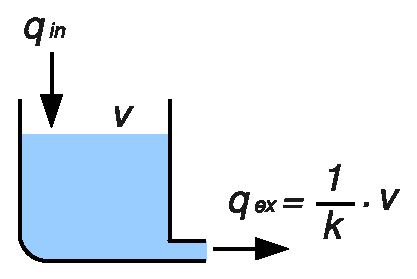
\includegraphics[width=0.4\columnwidth]{\figdir/classDef_linearReserv/linReserv.eps}
  \caption{Sketch of a single linear reservoir. \label{eqn:concept-classDef-linReserv-sketch}}
\end{figure}

The ordinary differential equation that results from combining \eqnsref{eqn:concept-classDef-linReserv-continuity} and \ref{eqn:concept-classDef-linReserv-outflow} can be solved analytically. With the simplest assumption of a constant inflow rate $q_{in}$ over a time step of length $\Delta t$ the integration yields \eqnref{eqn:concept-classDef-linReserv-solution-v}, where $v(t_0)$ is the initial storage at time $t_0$.

\begin{equation} \label{eqn:concept-classDef-linReserv-solution-v}
v(t_0 + \Delta t) = \left( v(t_0) - q_{in} \cdot k \right) \cdot e^{(-\Delta t/k)} + q_{in} \cdot k
\end{equation}

Using \eqnref{eqn:concept-classDef-linReserv-outflow} one can also transform \eqnref{eqn:concept-classDef-linReserv-solution-v} into an expression for the outflow rate $q_{ex}$ (\eqnref{eqn:concept-classDef-linReserv-solution-q}).

\begin{equation} \label{eqn:concept-classDef-linReserv-solution-q}
q_{ex}(t_0 + \Delta t) = \left( q_{ex}(t_0) - q_{in} \right) \cdot e^{(-\Delta t/k)} + q_{in}
\end{equation}

%%%%%%%%%%%%%%%%%%%%%%%%%%%%%%%%%%%%%%%%%%%%%%%%%%%%%%%%%%%%%%%%%%%%%%%%%%%%%%%%
\subsection{Step 1: Declaration of the class} \label{sec:concept-classDef-declaration}

To declare a new class, the model developer simply needs to specify the class' \emph{data members} (recall \secref{sec:concept-classFeatures-overview}). With respect to the example of the linear reservoir (\secref{sec:concept-classDef-linReserv}), one would have to declare
\begin{itemize}
  \item a single scalar state variable (storage volume $v$).
  \item a single scalar parameter (retention constant $k$). We assume here that this parameter is object-specific, \ie{} each linear reservoir has an individual $k$.
  \item a single input variable (inflow rate $q_{in}$). We assume here that this is a simulated input rather than an external input (recall \secref{sec:concept-classFeatures-inputs}).
  \item a single output variable (outflow rate $q_{ex}$)
\end{itemize}

As described in \secref{sec:concept-autocode-codegen-input}, this information has to be collected in a table-formatted text file for later processing by the code generator (\secref{sec:concept-classDef-codegen}). An appropriate input file for the code generator is shown in \figref{fig:concept-classDef-declaration-example}.

\begin{figure}[htb]
  \lstinputlisting[style=txt,linewidth=\columnwidth]{\figdir/classDef_linearReserv/declaration.txt}
  \caption[Input file for the code generator, containing the declaration of a linear reservoir class.]{Input file for the code generator, containing the declaration of a linear reservoir class. See \tabref{tab:concept-featuretypes} for the entries allowed in the 'type' column. \label{fig:concept-classDef-declaration-example}}
\end{figure}

%%%%%%%%%%%%%%%%%%%%%%%%%%%%%%%%%%%%%%%%%%%%%%%%%%%%%%%%%%%%%%%%%%%%%%%%%%%%%%%%
\subsection{Step 2: Code generation} \label{sec:concept-classDef-codegen}

Once all data members of all classes have been declared in the required form (see \secref{sec:concept-autocode-codegen-input} and \figref{fig:concept-classDef-declaration-example}), the table is further processed by the code generator\index{code generator}. Assuming that the contents of \figref{fig:concept-classDef-declaration-example} is saved in a file 'linRes.txt', an appropriate call to the code generator could be:

\begin{lstlisting}[style=R]
library("codegen")
generate(
  files=c(linReserv="linRes.txt"),
  outdir="generated_code"
  overwrite=TRUE
)
\end{lstlisting}

Note that the vector of class declaration files passed to the \texttt{files} argument must have as many elements as there are classes in the model. In our minimum example with only a single class, this vector is of lenght 1. Also note that this must be a \emph{named} vector because the class' names are generated from the elements' names. Thus, the name for the linear reservoir class would be 'linReserv' in the above example.

The complete output from the above call to the \texttt{generate} method is not presented here. An an overview of the created files was already given in \secref{sec:concept-autocode-codegen-output} and a central part of the generated code is shown in \figref{fig:concept-classDef-methodsFrame}.

%%%%%%%%%%%%%%%%%%%%%%%%%%%%%%%%%%%%%%%%%%%%%%%%%%%%%%%%%%%%%%%%%%%%%%%%%%%%%%%%
\subsection{Step 3: Implementing the class' methods} \label{sec:concept-classDef-simulate}

As mentioned in \secsref{sec:concept-autocode-role} and \ref{sec:concept-autocode-codegen-output}, the implementation (\ie{} the body code) of the 'simulate' and 'derivsScal' methods has to be provided by the model developer. The code generator only creates appropriate method interfaces and include statements. For the linear reservoir class introduced in \secref{sec:concept-classDef-linReserv}, part of the generated code is shown in \figref{fig:concept-classDef-methodsFrame}.

\begin{figure*}
  \lstinputlisting[style=c++, framexleftmargin=0mm, numbers=left, stepnumber=1, numbersep=2mm, numberstyle=\ttfamily\footnotesize, firstline={40}] {\figdir/classDef_linearReserv/AUTOechse_userClass_linReserv.h}
  \caption{Part of the generated header file for the linear reservoir class showing the frame of the 'simulate' and 'derivsScal' methods. The manually written code is imported by the \texttt{\#include} directives. \label{fig:concept-classDef-methodsFrame}}
\end{figure*}

Two complete, alternative bodys of the 'simulate' and 'derivsScal' methods of the linear reservoir class are presented in  \figref{fig:concept-classDef-implementation-analytical} \& \ref{fig:concept-classDef-implementation-numerical}. This is the code which would be imported by the \verb!#include! directives in \figref{fig:concept-classDef-methodsFrame}.

\begin{figure*}
  File '\verb!userCode_linReserv_aux.cpp!'
  \lstinputlisting[style=c++, framexleftmargin=0mm, numbers=left, stepnumber=1, numbersep=2mm, numberstyle=\ttfamily\footnotesize]{\figdir/classDef_linearReserv/userCode_linReserv_analytical-aux.cpp}
  File '\verb!userCode_linReserv_simulate.cpp!'
  \lstinputlisting[style=c++, framexleftmargin=0mm, numbers=left, stepnumber=1, numbersep=2mm, numberstyle=\ttfamily\footnotesize]{\figdir/classDef_linearReserv/userCode_linReserv_analytical-simulate.cpp}
  File '\verb!userCode_linReserv_derivsScal.cpp!'
  \lstinputlisting[style=c++, framexleftmargin=0mm, numbers=left, stepnumber=1, numbersep=2mm, numberstyle=\ttfamily\footnotesize]{\figdir/classDef_linearReserv/userCode_linReserv_analytical-derivsScal.cpp}
  \caption[Bodies of the 'simulate' and 'derivsScal' methods for the linear reservoir class if an analytical solution is adopted.]{Bodies of the 'simulate' and 'derivsScal' methods for the linear reservoir class if an analytical solution is adopted. \label{fig:concept-classDef-implementation-analytical}}
\end{figure*}

\begin{figure*}
  File '\verb!userCode_linReserv_aux.cpp!'
  \lstinputlisting[style=c++, framexleftmargin=0mm, numbers=left, stepnumber=1, numbersep=2mm, numberstyle=\ttfamily\footnotesize]{\figdir/classDef_linearReserv/userCode_linReserv_numerical-aux.cpp}
  File '\verb!userCode_linReserv_simulate.cpp!'
  \lstinputlisting[style=c++, framexleftmargin=0mm, numbers=left, stepnumber=1, numbersep=2mm, numberstyle=\ttfamily\footnotesize]{\figdir/classDef_linearReserv/userCode_linReserv_numerical-simulate.cpp}
  File '\verb!userCode_linReserv_derivsScal.cpp!'
  \lstinputlisting[style=c++, framexleftmargin=0mm, numbers=left, stepnumber=1, numbersep=2mm, numberstyle=\ttfamily\footnotesize]{\figdir/classDef_linearReserv/userCode_linReserv_numerical-derivsScal.cpp}
  \caption[Bodies of the 'simulate' and 'derivsScal' methods for the linear reservoir class if a numerical solution is adopted.]{Bodies of the 'simulate' and 'derivsScal' methods for the linear reservoir class if a numerical solution is adopted. Note that the value of the volume state variable ($v$) in the 'derivsScal'method is accessed via \texttt{u[INDEX\_v]} instead of \texttt{stateScal(v)}. \label{fig:concept-classDef-implementation-numerical}}
\end{figure*}

%%%%%%%%%%%%%%%%%%%%%%%%%%%%%%%%%%%%%%%%%%%%%%%%%%%%%%%%%%%%%%%%%%%%%%%%%%%%%%%%
\subsection{Step 4: Compilation} \label{sec:concept-classDef-compile}

Once the code generator has run successfully and the methods for all classes are implemented, the application specific simulation software (\ie{} the 'model engine') has to be build. This is achieved by compiling and linking all parts of the source code, namely
\begin{enumerate}
  \item the static part of the code, providing the basic infrastructure for every model.
  \item the application-specific code created by the code generator (see \secref{sec:concept-classDef-codegen}).
  \item the body code of the 'simulate' and 'derivsScal' methods, manually written by the model developer.
\end{enumerate}

The GNU C++ compiler is used for this purpose and the procedure has been successfully tested on several platforms. To assist the developer in the compilation process, platform-specific makefiles are available.

If invalid code is detected in the manually written parts of the code, the compilation will fail, of course and one has to go through the usual steps of debugging. One should keep in mind, however, that a successful compilation does not necessarily mean that the code is 'correct' in the sense that it produces the desired results. The correctness of the code can only be verified by analyzing the model's output.

%%%%%%%%%%%%%%%%%%%%%%%%%%%%%%%%%%%%%%%%%%%%%%%%%%%%%%%%%%%%%%%%%%%%%%%%%%%%%%%%
%%%%%%%%%%%%%%%%%%%%%%%%%%%%%%%%%%%%%%%%%%%%%%%%%%%%%%%%%%%%%%%%%%%%%%%%%%%%%%%%
%%%%%%%%%%%%%%%%%%%%%%%%%%%%%%%%%%%%%%%%%%%%%%%%%%%%%%%%%%%%%%%%%%%%%%%%%%%%%%%%

\FloatBarrier

\section{Outline of computational steps} \label{sec:concept-compSteps}

\subsection{Overview} \label{sec:concept-compSteps-overview}

The essential computational steps carried out when executing a model are summarized in \figref{fig:concept-compSteps}. Note that this outline applies to \emph{any} model built with the \software{echse} simulation environment.

\begin{figure}[h]
\smallskip
\textit{Main function} \\
\colorbox{shadecolor}{
\begin{minipage}{0.95\columnwidth}
  \smallskip
  \begin{itemize}
    \item Retrieval of command line arguments (\secref{sec:input-commandline})
    \item Reading of the configuration file (\secref{sec:input-config})
    \item Instantiation of objects \& object groups (see \figref{fig:concept-terms_implementation})
    \item Initialization of the objects' data.
  \end{itemize}
  \smallskip
    \textit{Loop over time steps} \\
    \framebox{
    \begin{minipage}{0.9\columnwidth}
      \smallskip
      \begin{itemize}
         \item Updating of external inputs
      \end{itemize}
      \smallskip
      \textit{Loop over objects} \\
      \framebox{
      \begin{minipage}{0.85\columnwidth}
        \smallskip
        \begin{itemize}
           \item Call of the 'simulate' method for current object
        \end{itemize}
      \end{minipage}
      }
      \begin{itemize}
         \item Writing of data to output files
      \end{itemize}
    \end{minipage}
    }
    \begin{itemize}
      \item Closing of output files
    \end{itemize}
  \begin{itemize}
    \item Clean-up
    \item Output of traceback info in case of exceptions
    \item Setting of return code and termination
  \end{itemize}
\end{minipage}
}
  \caption[Essential computational steps of a model run.]{Essential computational steps of a model run. The framed boxes represent loops, thus the tasks inside these boxes are executed repeatedly (see \secref{sec:concept-compSteps-loopNesting}). \label{fig:concept-compSteps}}
\end{figure}

Most of the computational steps listed in \figref{fig:concept-compSteps} appear in any dynamic systems simulation software. Only those aspects which are specific to \software{echse} models are discussed in the subsequent sections.

\subsection{Time and object loop} \label{sec:concept-compSteps-loopNesting}

In \figref{fig:concept-compSteps}, the innermost framed box represents the so-called \emph{object loop}. The purpose of this loop to iterate through all objects and trigger the simulation for a single time step by calling the objects' 'simulate' methods (see \secref{sec:concept-classFeatures-simulateMethod}). In a spatially distributed model, the term 'spatial loop' is often an appropriate synonym for 'object loop'\footnote{In the current version of the software, the object loop is split into two nested loops to enable parallel processing. This is not essential for the understanding for the general understanding, however.}.

Note that the \emph{time loop} is wrapped around the object loop (\figref{fig:concept-compSteps}). This design can be found in virtually all spatially distributed models that solve \emph{partial} differential equations (PDE) such as groundwater flow models or hydrodynamic models. Note, however, that a few models exist where the two loops are in reverse order, for example in some hydrological catchment models.

The consequence of having the object loop \emph{inside} the time loop is that, for a particular time step, the 'simulate' method is executed for \emph{all} objects, before the computation proceeds with the subsequent time step. This allows for the exchange of information between objects in every single time step. This is a precondition for properly handling \emph{feedbacks} between objects, \ie{} two-way interactions (see \figref{fig:concept-interactions-types}, \secref{sec:concept-interactions-types}).

The only drawback of this approach is the requirement of keeping instances of \emph{all} objects in memory at the same time. Thanks to the large memory capacity of modern computers, this is hardly an issue. If the number of objects should actually be too large to fit into memory, a cheap solution would be to split the model (into spatial sub-domains, for example) in a way that no feedback between the sub-models does occur.

\subsection{Exception handling} \label{sec:concept-compSteps-exceptionHandling}

In a complex and flexible software it is not unlikely that an unrecoverable error occurs during computations. The potential causes are manifold, ranging from missing or erroneous input data to mathematical calculations yielding invalid results (NaN, Inf, ect.).

The models built with the \software{echse} simulation environment use C++'s exceptions\index{exceptions} mechanism to handle situations like that. Whenever an exception occurs, the normal execution of the program is suspended and priority is given to exception handling. In the case of \software{echse} models, this means that the currently active unit (\ie{} a class method or function) tries to collect as many information as possible about the circumstances of the exception and then gives control back to its calling unit. The calling unit behaves just like the unit where the exception originally occurred. In this way, the error signal is passed through the hierarchy of routines and finally causes an exception at the highest level, the 'main' function. Here (and only here), traceback\index{traceback} information is generated and the program is forced to terminate (see final step in \figref{fig:concept-compSteps}).

The traceback always contains (for every unit) information about
\begin{enumerate}
  \item the name of the unit, where the exception occurred.
  \item a description of the circumstances and possibly the cause of the exception.
  \item the name of the source file containing the unit that failed.
  \item the line of this file where the exception was thrown.
\end{enumerate}

Based on the traceback information, the location and cause of the error can usually be  identified with little effort.

If the model terminated due to an exception, the program issues a non-zero return code. If no exception occurred, a the code of zero is returned as this is widely used convention. The return code should always be checked if the model is embedded in another software such as a scripts or batch files.

%%%%%%%%%%%%%%%%%%%%%%%%%%%%%%%%%%%%%%%%%%%%%%%%%%%%%%%%%%%%%%%%%%%%%%%%%%%%%%%%
%%%%%%%%%%%%%%%%%%%%%%%%%%%%%%%%%%%%%%%%%%%%%%%%%%%%%%%%%%%%%%%%%%%%%%%%%%%%%%%%
%%%%%%%%%%%%%%%%%%%%%%%%%%%%%%%%%%%%%%%%%%%%%%%%%%%%%%%%%%%%%%%%%%%%%%%%%%%%%%%%

\section{Interactions between objects} \label{sec:concept-interactions}


\subsection{Overview and accessible data} \label{sec:concept-interactions-access}

Interactions \index{object!interaction}\index{interactions|see{object interaction}} between objects are a typical in natural and technical systems. In this context, an interaction is defined as an exchange of either matter (mass), energy, or information. Although it is possible to simulate just a single object or a group of non-interacting objects, interactions have to be considered in the vast majority of real-world models.

As already outlined in \secsref{sec:concept-classFeatures-inputs} and \ref{sec:concept-classFeatures-outputs}, an interaction between two objects is bound to the declaration of
\begin{enumerate}
  \item a \emph{simulated input variable} in the class corresponding to the object that \emph{uses} data provided by another object.
  \item an \emph{output variable} in the class corresponding to the object that \emph{provides} the data to be used by (an)other object(s).
\end{enumerate}

In a dynamic simulation model with sequential processing of the objects (see \secref{sec:concept-compSteps-loopNesting} and \figref{fig:concept-compSteps}), further limitations with respect to the acessibility of data do exist. This is illustrated in \figref{fig:concept-interactions-access} from the perspective of a single object with respect to a single time step (bold-framed object $M_k$). Assuming that appropriate simulated input and output variables have been declared in the respective classes (see above), for the simulation of time step $i$, the object $M_k$ has access to
\begin{enumerate}
  \item data on the object itself, representing the state at the end of the previous time step with index $i-1$.
  \item the output variables of the already processed \emph{upstream} objects. These values are representative for the end of the \emph{current} time step ($i$).
  \item the output variables of the \emph{downstream} objects still waiting for being simulated. These values are representative for the end of the \emph{previous} time step ($i-1$).
\end{enumerate}

\begin{figure}
  \centering
  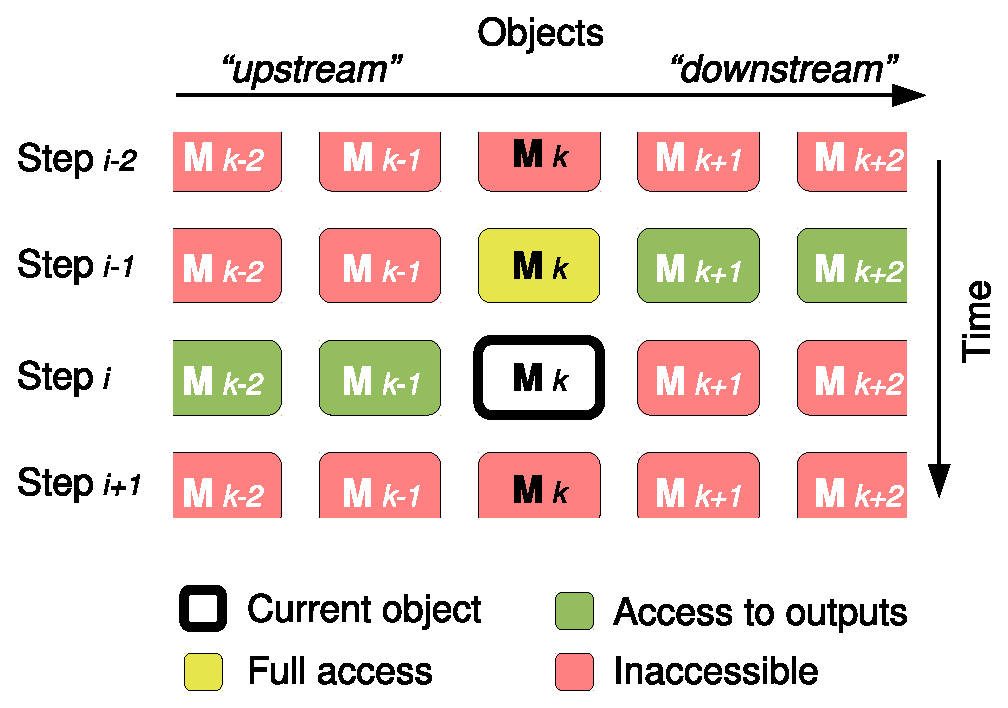
\includegraphics[width=0.9\columnwidth]{\figdir/interactions/interactions_access.eps}
  \caption{Accessible data from a single object's perspective. \label{fig:concept-interactions-access}}
\end{figure}

\subsection{Types of interactions} \label{sec:concept-interactions-types}

Looking at two interacting objects, one generally has to distinguish between \emph{feed-forward} interactions (also called \emph{one-way} interactions) and \emph{feedbacks}, also known as \emph{two-way} interactions (\figref{fig:concept-interactions-types}). The difference between the two is illustrated also in \figref{fig:concept-interactions-bucketExample} on a very simple example. Typical real-world examples of feedbacks in the field of hydrology include
\begin{itemize}
  \item interactions between river and floodplain. River stage and groundwater level are coupled via inflitration and leakage, respectively.
  \item diffusion problems at the interface of the pelagic and benthic zone. The rate of diffusive transport depends on both, the concentration in the water body and the sediment's pore water.
  \item the operational control of a reservoir's outflow based on stream flow data observed at a gage downstream of the reservoir.
\end{itemize}

\begin{figure}
  \centering
  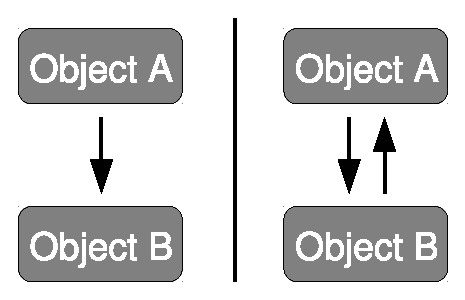
\includegraphics[width=0.5\columnwidth]{\figdir/interactions/interactions_types.eps}
  \caption[Basic types of object interaction.]{Basic types of object interaction. The arrows indicate exchange of matter, energy, or information. Left: Feed-forward type. Right: Feedback type. \label{fig:concept-interactions-types}}
\end{figure}

\begin{figure}
  \centering
  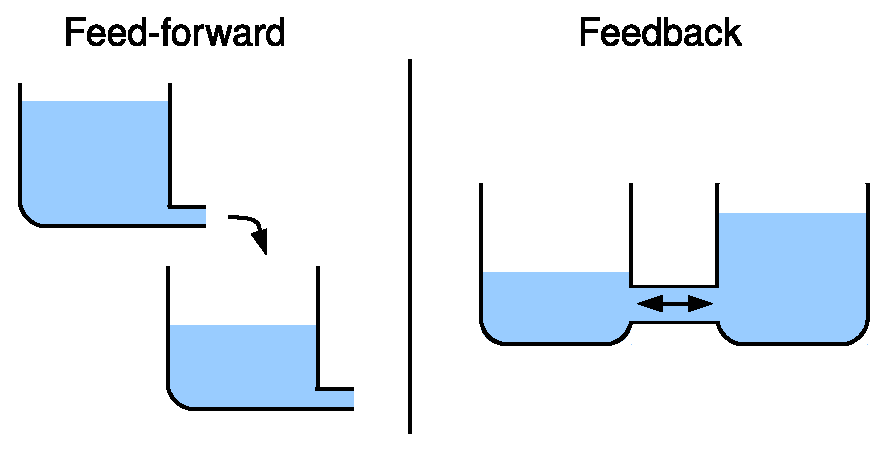
\includegraphics[width=0.75\columnwidth]{\figdir/interactions/interactions_buckets.eps}
  \caption{Types of interactions between two buckets filled with a liquid. \label{fig:concept-interactions-bucketExample}}
\end{figure}

The feedback (\figsref{fig:concept-interactions-types} \& \ref{fig:concept-interactions-bucketExample}, right) represents the more general type of interaction and, actually, the feed-forward interaction (\figsref{fig:concept-interactions-types} and \ref{fig:concept-interactions-bucketExample}, left) may be regarded just as a special type of (missing) feedback. It makes sense, however, to strictly distinguish between the two types of interaction in the context of dynamic simulation, \ie{} when modeling the interaction of objects over a sequence of discrete time steps. This is due to the following:

\begin{description}
  \item [Feed-forward type] As long as the exchange of data between two interacting objects 'A' and 'B' is effectively \emph{one-way}, the two objects can be simulated \emph{sequentially}, \ie{} one after another. The so-called \emph{source object} ('A' in \figref{fig:concept-interactions-types}, left) represents the 'data provider' and must be simulated first. The output of 'A' is then used as an input for the \emph{target object} ('B'), which is simulated later.
  \item [Feedback type] If there is a \emph{two-way} exchange of data between two objects 'A' and 'B', these objects must be simulated \emph{simultaneously}, \ie{} at the same time. To put it in other words: The ordinary differential equations, describing the evolution of the state variables in object 'A' form a coupled system with the equations of object 'B'. To get a proper solution, the coupled differential equations must be integrated simultaneously using an ODE solver \citep[see \eg{}][]{Press2002}. This, however, conflicts with the facts that (1) objects are geberally treated as well-separated entities and (2) the array of objects is processed sequentially using a fixed order (see innermost loop in \figref{fig:concept-compSteps}). Nevertheless, \software{echse}-based models are capable of handling feedback interactions using the techniques outlined in \secref{sec:concept-interactions-feedbackHandling}.
\end{description}

\subsection{Handling of feedbacks} \label{sec:concept-interactions-feedbackHandling}

\subsubsection*{Option 1: Compound classes}

A straightforward approach to cope with the problem of feedback interactions (\secref{sec:concept-interactions-types}) is to avoid inter-object feedbacks. Taking the objects 'A' and 'B' from \figref{fig:concept-interactions-types} (right) as an example, this would mean that the class(es), of which the objects 'A' and 'B' are instances, are joined to form a new (compound) class. The feedback interaction between the former objects 'A' and 'B' is then \emph{internally} present in an object of the compound class. The coupled differential equations related to all state variables (which were originally distributed over object 'A' and 'B') can then be solved simultaneously using a standard ODE solver within the simulate method (\secref{sec:concept-classFeatures-simulateMethod}) of the compound class.

The drawback of such an approach is that the compound class may quickly become rather complex. In extreme cases of many feedback interactions, one might end up with a model consisting of only a single object being an instance of a single class which basically integrates 'everything'. In such a case one should think about other strategies (see below) or use another, more appropriate modeling software.

\subsubsection*{Option 2: Step-wise feedback}

The simplest and probably the most common solution for the feedback problem is to treat the differential equations in the two interacting objects 'A' and 'B' as \emph{temporarily independent}. In practice, this works as follows:
\begin{description}
  \item [Simulation step] The objects 'A' and 'B' are simulated independendly, as if there was no interaction at all. This means that the state variables of 'A' and 'B' are updated by separately integrating the respective differential equations.
  \item [Feedback step] After \emph{every} time step, the two objects exchange information about their new states. The information about 'A' is then used in the subsequent simulation step for 'B' and vice versa.
\end{description}

To make the described approach of \emph{step-wise feedback} successfully work in practice, two conditions must be met.

Firstly, the interacting objects 'A' and 'B' must exchange data with a high frequency. This is achieved by running the simulation in small time steps. The longer the time step, the higher the potential numerical error will be.

Secondly, it has to be ensured that the information about object 'B' used by 'A' refers to the \emph{same point in time} as the information about 'A' used by 'B'. In a normal sequential simulation, where either 'A' or 'B' is processed first, this is not the case. However, with the help of a so-called \emph{observer object} it is possible to supply 'A' and 'B' with data of equal up-to-dateness, in spite of sequential processing. This strategy is illustrated by \figref{fig:concept-interactions-observer}. In the shown example, a feedback interactions exists between the objects $M_k$ and $M_{k+1}$. The role of the auxiliary observer object $M_{k-1}$ is to collect data on $M_k$ and $M_{k+1}$ which is representative for a particular point in time, namely the (end of) time step $i-1$. The collected information is then supplied to $M_k$ and $M_{k+1}$, respectively, to be used in the simulation over the current time step $i$.

\begin{figure}
  \centering
  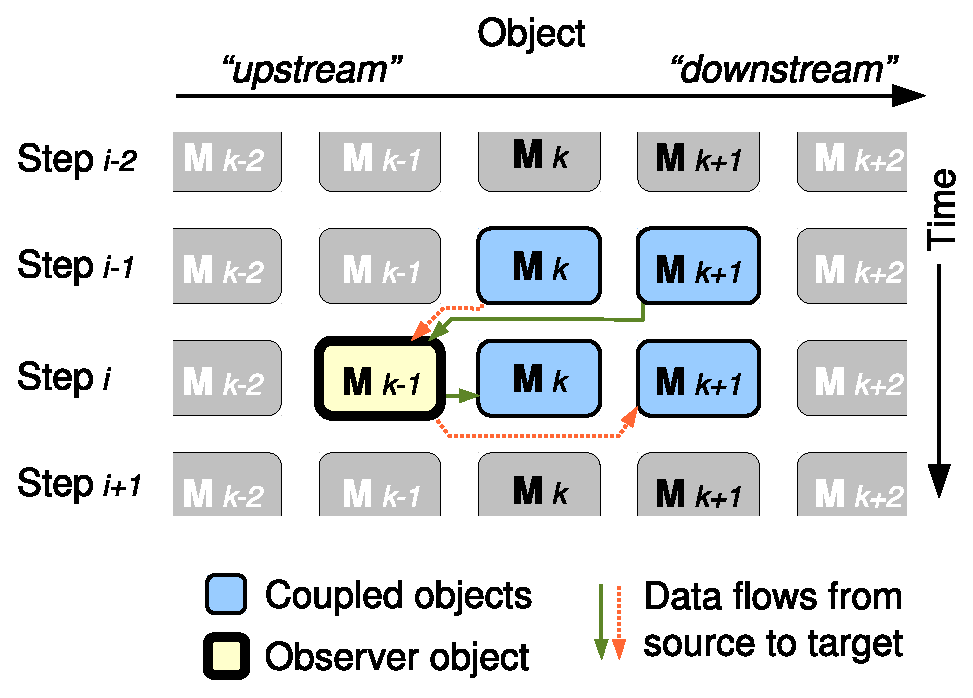
\includegraphics[width=0.9\columnwidth]{\figdir/interactions/interactions_observer.eps}
  \caption{Use of an artificial \emph{observer object} to provide two sequentially processed, feedback-coupled objects with information of equal up-to-dateness. \label{fig:concept-interactions-observer}}
\end{figure}

\subsubsection*{Step-wise feedback: Time step issues}

As mentioned above, the selection of a sufficiently short time steps is necessary to keep the error associated with the step-wise handling of feedbacks within acceptable limits. A disadvantage of the current version of the \software{echse} is that the time step is a fixed parameter. Consequently, if a short time step is selected with the intention of increasing the accuracy of feedback solutions, the computation will slow down even for those objects which are not subject to feedback interactions. Thus, a single feedback interaction may impact negatively on the performance of the entire model in terms of computation time. A possible solution to this problem lies in releasing the constraints of the fixed 'global' time step. In particular, it would make sense allow a variable number of sub-steps to be specified for each object. The only restriction would be that the number of sub-steps must be identical for two objects having a feedback relation. If a feedback interaction exists between two objects 'A' and 'B' and another one exists between two objects 'C' and 'D', the number sub-steps applied to the first group ('A', 'B') and the second group ('C', 'D') may still be different, however. It is planned to implement the sub-step approach in an upcoming version of the \software{echse}.

\subsubsection*{Step-wise feedback: Accuracy}

To really understand the limits of the strategy of a step-wise simulation of feedbacks, a closer look on the solution strategy is required. Let's take the example of \figref{fig:concept-interactions-observer}, where a feedback interaction between the objects $M_k$ and $M_{k+1}$ is simulated under the control of an observer object $M_{k-1}$. In a first step, the observer object $M_{k-1}$ collects information from both object $M_k$ and $M_{k+1}$ which is representative for time step $i-1$. If the objects $M_k$ and $M_{k+1}$ were the two connected buckets shown in the right column of \figref{fig:concept-interactions-bucketExample}, the observer $M_{k-1}$ would collect information on the water levels in the two buckets and compute the resulting flow rate. Then, the two objects $M_k$ and $M_{k+1}$ would retrieve the computed flow rate from the observer and both objects would use this information to calculate their individual water levels at the end of time step $i$.

It is important to realize that the accuracy of the resulting solution is limited by the fact that the information on the flow rate between the two buckets is a contant. This rate effectively represents the sitution at the end of time step $i-1$ or (in other words) the situation at the \emph{very beginning} of time step $i$. This \emph{constant} information is then used in the simulation of the \emph{entire} time step $i$, neglecting that the water levels change, hereby affecting the flow rate.

Solutions with these characteristics are also called \emph{Euler solutions}. It is well known that the accuracy of such first-order solutions is quite limited. Therefore, with the current version of the \software{echse} a reasonable simulation of feedbacks can only be expected if
\begin{itemize}
  \item non-linearities are weak.
  \item the chosen simulation time step is sufficiently short.
\end{itemize}

A straighforward method to examine the accuracy of the simulation of feedback interactions is to simply run the model with different time steps and to compare the results for the affected objects. It is possible that support for higher-order solutions (Heun, Runge-Kutta, etc.) and/or methods of automatic time step control will be implemented in a future version of the \software{echse}.

\subsection{Conservation of mass or energy}

As explained earlier, information is not continuously exchanged between interacting objects but only after discrete time steps. This is true for both feed-forward and feedback interactions. In the usual case of non-linear dynamics, it is quite important to understand the consequences with respect to the loss of accuracy and regarding the conservation of mass or energy in particular.

Recall the example of the two separate buckets shown at the left side of \figref{fig:concept-interactions-bucketExample}. In this feed-forward interaction, the bucket at the bottom receives inflow from the other bucket. If we assume that the upper bucket has the characteristics of a linear reservoir (see \secref{sec:concept-classDef-linReserv}) we known from \eqnref{eqn:concept-classDef-linReserv-solution-q} (page \pageref{eqn:concept-classDef-linReserv-solution-q}) that the outflow is a \emph{non-linear} (exponential) function of time (\figref{fig:concept-interactions-accuracy}).

\begin{figure}
  \centering
  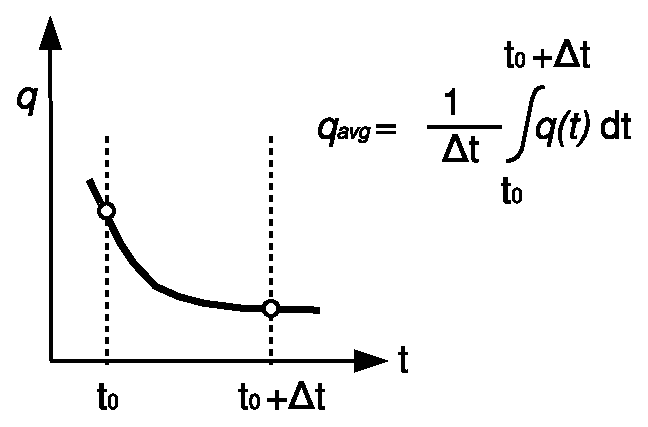
\includegraphics[width=0.6\columnwidth]{\figdir/interactions/interactions_accuracy.eps}
  \caption{Example outflow $q$ from a linear reservoir within a discrete modeling time step of length $\Delta t$. \label{fig:concept-interactions-accuracy}}
\end{figure}

Recalling \secref{sec:concept-classFeatures-outputs}, we know that all information about the upstream bucket's outflow needs to be passed to the downstream bucket through output variables. Often, the crux for the model developer is to define the output variables in way that
\begin{enumerate}
  \item the information on the dynamics is retained.
  \item mass (or energy) is conserved.
\end{enumerate}

Unfortunately, these two goals cannot be achieved at the same time and one needs to set a priority. Based on the example from \figref{fig:concept-interactions-accuracy}, some possible options are discussed in the following.

\subsubsection*{Boundary values}

A simple solution would be to pass the values at time step boundaries through two output variables:
\begin{itemize}
  \item The flow rate at the beginning of the time step $q(t_0)$.
  \item The flow rate at the end of the time step $q(t_0 + \Delta t)$.
\end{itemize}

In this way, at least the information on the change of the flow rate within the time step is retained. However, the information on the actual non-linearity is lost. Consequently, the information on the true cumulated outflow, \ie{} the exchanged volume, is lost too.

\subsubsection*{'Improper' average}

Another option would be to pass only an average outflow rate computed as the arithmetic mean of $q(t_0)$ and $q(t_0 + \Delta t)$. In most cases, this is not recommended, because neither of the two above-mentioned goals is met. Firsty, the information on the dynamics is completely lost. Secondly, use of the average value as defined above results in a mass balance error if the true dynamics is \emph{non-linear}. This is true in the example (\figref{fig:concept-interactions-accuracy}) as well as in most real-world situations.

\subsubsection*{Intermediate values}

With this strategy, information on the outflow at intermediate times is passed. For example, one could pass the 3 values $q(t_0)$, $q(t_0 + 1/2 \Delta t)$, $q(t_0 + \Delta t)$. Then, the downstream bucket could try to re-construct the non-linear dynamics, for examply by fitting an interpolation function $g(t)$ to the three values.

\subsubsection*{Interpolation parameters}

This is just a special case of the afore-mentioned option. In this case, one does not pass the outflow rates at intermediate times. Instead, the parameters of the interpolation function $g(t)$ are passed. Depending on the specific case and the type of the interpolation function, this may reduce the number of necessary output variables.

\subsubsection*{'Proper' time-step average}

If the priority is on conservation of mass, one needs to pass a \emph{proper} average outflow rate $\overline{q_{out}}$ from the upstream to the downstream bucket. The two above-mentioned approaches allow for the calculation of an approximate average outflow rate as

\begin{equation*}
  \overline{q_{out}} \approx \frac{1}{\Delta t}\int_{t_0}^{t_0+\Delta t}g(t)
\end{equation*}

with $g(t)$ being the interpolation function. To make this work in practice, the interpolation function $g(t)$ must be integratable and allow for a reasonable fit of the dynamics.

Another strategy which is often more straightforward is based on a discrete mass balance for the upstream bucket. Denoting the volume of the upstream bucket as $v$ and assuming a \emph{constant} inflow rate $q_{in}$, the time-step averaged outflow rate $\overline{q_{out}}$ is

\begin{equation*}
  \overline{q_{out}} = q_{in} - \frac{v(t_0 + \Delta t) - v(t_0)}{\Delta t}
\end{equation*}

The approach remains applicable even if more input or loss terms appear in the bucket's mass balance. It is not even necessary that these terms are constant over the time step of length $\Delta t$, but then, their cumulated values (integrals over $\Delta t$) must be known. In practice, these integral values can be obtained by introducing auxiliary state variables representing the cumulated inputs and/or losses. These auxiliary state variables can be initialized with zero at the begin of each time step.

\subsubsection*{Combined approaches}

In some cases, it may be favourable to combine some of the approaches discussed above. For example, one could pass the values at the time-step boundaries as well as the proper time-step average value. In this way, the loss of information at the interface between the interacting objects is minimized.
